\section{Introduction}

The Volterra series provides a linear-in-the-parameters representation for a broad class of nonlinear systems, however we have seen in Chapter \ref{sec:RegVolterraTD} that the estimation of its associated Volterra kernels is ill-suited to a standard least squares framework. This is because the nonparametric nature of the model implies a requirement for large numbers of parameters, which in turn produces large variances in least squares estimates obtained from a finite and noisy data record. 

In order to reduce the variance of kernel estimates, a regularized least squares approach was developed in \cite{Birpoutsoukis2017} and \cite{Birpoutsoukis2017c}. As discussed in Chapter \ref{chap:3}, the method uses Bayesian techniques to impose smoothness and decay along the (hyper)surfaces of each Volterra kernel, which is a nonlinear extension of Bayesian impulse response identification as introduced in \cite{Pillonetto2010}. The regularized estimation employs a set of tunable hyperparameters to describe the smoothness and decay rates of each kernel, where traditionally such hyperparameters have been optimized through a maximization of the associated marginal likelihood expression, which is typically non-convex \cite{Chen2013}. The dimension of the search space for this optimization increases quadratically with the order of the Volterra series model, since decay hyperparameters are required for each dimension of each kernel.

When compared to standard least squares and other more traditional estimation methods, the main disadvantages of the regularization approach in \cite{Birpoutsoukis2017} are:
\begin{itemize} 
\item Increased computational cost,
\item Poor computation time scaling with the maximum series order, $M$,
\item Risk of converging to a local minimum in the hyperparameter optimization 
\end{itemize}
These disadvantages are directly acknowledged in the concluding remarks of \cite{Birpoutsoukis2017}, which states:
\begin{quote}
``Several issues should be addressed in the future, such as efficient ways to optimize the hyperparameters of the regularization matrix in order to reduce the risk of resulting in a local minimum of the marginal likelihood.''
\end{quote} 

To address the issues of computation time scaling and non-convexity, an alternative hyperparameter tuning method is developed in this chapter. The new method is proposed within the expectation-maximization (EM) framework \cite{Dempster1977}, and is inspired by results from \cite{Bottegal2015} and \cite{Bottegal2016} which deal with linear system identification. When applied to Volterra series estimation, the approach will be shown to trade the single large optimization problem in \cite{Birpoutsoukis2017} for a set of smaller problems in an iterative scheme, where the maximum dimension of the search space increases linearly with the series order. 

Numerical examples in Section \ref{sec:NumEx_EM} confirm that computation times for the EM-based formulation do not increase as rapidly with series order, while still converging to the same hyperparameters as the marginal likelihood optimization traditionally used in these problems.

\section{The expectation-maximization algorithm}

`Expectation-maximization' refers to a family of computation methods designed to find maximum likelihood estimates in cases where there are latent (unobserved) variables \cite{McLachlan2007}. These latent variables may represent real unobserved data, or (as is the case in this thesis) they can be `nuisance parameters' resulting from the reformulation of an estimation problem. 

In the general case, consider a data vector, $X$, which is a concatenation of two subvectors:
\begin{equation}
X = \begin{bmatrix} Y \\ Z \end{bmatrix},
\end{equation}
where $Y$ is the vector of \emph{observed} data, while $Z$ represents the \emph{unobserved} variables. Assume further that $X$ is drawn from some distribution, $p_c(Y,Z ; \eta)$, which is described by the unknown parameters, $\eta$. Under these conditions, the maximum likelihood estimation of $\eta$ is the problem of interest, i.e.
\begin{equation}
\hat{\eta} = \text{arg } \underset{\eta}{\text{max }} L_c(Y,Z ; \eta),
\label{eq:EM_jointlikelihoodopt}
\end{equation}
where $L_c(Y,Z ; \eta) = \log p_c(Y, Z; \eta)$ is the log likelihood function for the complete data vector, $X$. However since the $Z$ portion of data is not observed, (\ref{eq:EM_jointlikelihoodopt}) cannot be used directly.

One possible solution is to produce a marginal likelihood function by integrating out the latent variables from our distribution, yielding a marginal likelihood maximization (MLM) problem:
\begin{align}
\hat{\eta} &= \text{arg } \underset{\eta}{\text{max }} \log \int_Z p_c(Y,Z; \eta) \text{d}Z \\
&= \text{arg } \underset{\eta}{\text{max }} \log p(Y; \eta).
\label{eq:EM_marginallikelihoodopt}
\end{align}
Indeed, this is the typical pathway for regularized estimation problems employing empirical Bayes techniques \cite{Pillonetto2010}, \cite{Birpoutsoukis2017}, \cite{Lataire2016}.

There are many circumstances where a marginal likelihood approach becomes undesirable. For example, the marginalization process may be impossible or computationally intractable to perform, or it may be that the resultant optimization problem (\ref{eq:EM_marginallikelihoodopt}) is extremely difficult to solve. The latter problem is relevant to regularized Volterra series estimation, where the marginal likelihood approach implies searching through a high-dimensional non-convex function. In these situations, EM methods provide an alternate pathway which often resolves the issues associated with marginalization.

In essence, the EM approach moves back to the complete data problem, (\ref{eq:EM_jointlikelihoodopt}), but replaces the unobserved data, $Z$, with its expected value given $Y$ and some guess of $\eta$. While there is no reason to believe this guess is accurate, the procedure can be repeated iteratively with nice convergence properties for $\eta$. 

Conceptually, the iterative procedure for the EM method consists of two steps. The first is the \emph{expectation} step, where the complete data likelihood function is approximated using parameters, $\hat{\eta}^{(k)}$, from the previous iteration, i.e.
\begin{equation}
\label{estep}
Q(\eta,\hat{\eta}^{(k)}) = \textbf{E}\{  L_c(Y,Z;\eta) \},
\end{equation}
where $Q$ is the likelihood approximation, and the expectation is taken with respect to the posterior distribution $p(Z|Y; \hat{\eta}^{(k)})$.

The second step consists of a \emph{maximization}, where the parameters are updated by maximizing the function (\ref{estep}) calculated in the first step. The new hyperparameters are thus given by,
\begin{equation}
\hat{\eta}^{(k+1)} = \text{arg } \underset{\eta}{\text{max }} Q(\eta,\hat{\eta}^{(k)}).
\end{equation}

The chain of successive parameter estimates, $\hat{\eta}^{(k)}$, is called an \emph{EM sequence}, and there are some useful properties of this sequence which can be exploited. Noting first that $Q(\eta,\hat{\eta}^{(k)})$ is a lower bound on the marginal likelihood, $\log p(Y; \eta)$, it can be shown that each new iteration of the EM sequence corresponds to a higher point in the marginal likelihood function. If we impose the reasonable assumption that the marginal likelihood is itself upper bounded, then it is straightforward to show that the EM sequence will converge to a stationary point of $p(Y; \eta)$ \cite{Wu1983}. While some artificial examples have been constructed in the literature which converge to saddle points or local minima \cite{McLachlan2007}, a local maximum is almost guaranteed in practice. Thus, the EM method provides an alternate route to MLM without the need for explicit marginalization.

There is another property of the EM method which is not supported by formal results, but has been noted anecdotally. In comparison to standard MLM, the equivalent EM approach is often found to be more robust to poor initialization, and therefore less likely to settle in a sub-optimal local maximum. Such behaviour is particularly important in the Volterra series context, where MLM can involve many local maxima in the high-dimensional search space \cite{Birpoutsoukis2017}.

\section{Hyperparameter optimization using EM}

For the Bayesian estimation problem outlined in Chapter \ref{sec:RegVolterraTD}, the parameter vector, $\theta$, is framed as a random variable which is jointly distributed with the output data, $Y$. The problem of hyperparameter optimization can thus be framed as likelihood maximization with latent variables. The original parameter vector, $\theta$, becomes the unobserved data, and we require an estimate of all hyperparameters $\eta$ describing the joint distribution, i.e. 
\begin{equation}
\hat{\eta} = \text{arg } \underset{\eta}{\text{max }} L_c(Y,\theta;\eta),
\end{equation}
where $ L_c(Y,\theta;\eta)$ is the joint log likelihood of $Y$ and $\theta$.

This interpretation has already led to the MLM approach defined in (\ref{eq:MarginalLikelihood_opt}), both for the linear FIR and Volterra series cases. In this section, the EM solution will be derived for hyperparameter tuning in Volterra kernels with Gaussian priors. Relevant modeling assumptions will be (re)stated below for convenience.

\begin{assum}
The data generating model is a Volterra system with white Gaussian additive noise (\ref{eq:ReLS_VolterraModelStructure}), and uses the vectorized regression structure given in (\ref{eq:VolterraRegressionForm}), i.e.
\begin{equation}
\label{eq:VolterraRegressionForm_Chap4}
Y = \Phi^T \theta + E,
\end{equation}
with $\theta = [h_0, {h_1^\mathcal{V}}^T, {h_2^\mathcal{V}}^T, \hdots, {h_M^\mathcal{V}}^T]^T$.
\label{ass:ModelStructure_Chap4}
\end{assum}

\begin{assum}
The parameter vector is a Gaussian random variable, $\theta \sim \mathcal{N}(0,P)$, with block diagonal prior covariance (\ref{KernelPenalty}). Individual kernel covariances are defined using the TC structure, via (\ref{TCext}) and (\ref{FinalPenalty}).
\label{ass:GaussianTheta_Chap4}
\end{assum}

While the derivation is performed here for the TC covariance structure, the DC structure and others can be derived in an almost identical fashion.

\subsection{The expectation step}

Under assumptions \ref{ass:ModelStructure_Chap4} and \ref{ass:GaussianTheta_Chap4}, the lower bound function $Q(\eta,\hat{\eta}^{(k)})$ in (\ref{estep}) can be constructed analytically from the normal distributions of $Y$ and $\theta$. First, the function is separated into two components,
\begin{equation}
\label{Qsplit}
Q(\eta,\hat{\eta}^{(k)}) = \textbf{E}\{  \log p(Y|\theta; \eta) \} + \textbf{E}\{ \log p(\theta; \eta) \}.
\end{equation}
It can be seen from (\ref{eq:VolterraRegressionForm_Chap4}) that $Y|\theta;\eta \sim \mathcal{N}(\Phi^T \theta,\sigma^2I)$, hence,
\begin{align}
\textbf{E}\{  \log p(Y|\theta; \eta) \} &= \textbf{E} \{ a_1 - \frac{N}{2} \log \sigma^2 - \frac{1}{2 \sigma^2}(Y^T Y - 2 Y^T \Phi^T \theta + \theta^T \Phi \Phi^T \theta) \} \nonumber \\
&= a_1 - \frac{N}{2} \log \sigma^2 \label{qnoise} - \frac{1}{2 \sigma^2}\big(Y^T Y - 2 Y^T \Phi^T \textbf{E}\{\theta\} + \text{Tr}[\Phi \Phi^T \textbf{E}\{ \theta \theta^T \}]\big),
\end{align}
where $a_1$ is a real number, and $\sigma^2 \in \eta$ is the only hyperparameter present in the expression. The remaining expected values in (\ref{qnoise}) are taken with respect to $p(\theta|Y; \hat{\eta}^{(k)})$, with analytic expressions obtained via the joint distribution of $\theta$ and $Y$,
\begin{equation}
\begin{bmatrix}
\theta \\ 
Y
\end{bmatrix} \sim \mathcal{N} \Bigg(
\begin{bmatrix}
0\\ 
0
\end{bmatrix},
\begin{bmatrix}
P & P \Phi\\ 
\Phi^T P & \Phi^T P \Phi + \sigma^2 I 
\end{bmatrix} \Bigg).
\end{equation}
Using the standard expressions for Gaussian conditional distributions, and applying the matrix inversion lemma, we can arrive at numerically robust expressions for the desired expected values, 
\begin{align}
&\textbf{E} \{ \theta \} = \textbf{E} \{ \theta | Y \} = P(\hat{\eta}^{(k)}) [\Phi \Phi^T P(\hat{\eta}^{(k)}) + [\hat{\sigma}^2]^{(k)} I]^{-1} \Phi Y, \\
&\textbf{Cov} \{ \theta| Y \} = [\hat{\sigma}^2]^{(k)} P(\hat{\eta}^{(k)}) [\Phi \Phi^T P(\hat{\eta}^{(k)}) + [\hat{\sigma}^2]^{(k)} I]^{-1}, \\
&\textbf{E} \{ \theta \theta^T\} = \textbf{Cov} \{ \theta| Y \} + \textbf{E} \{ \theta | Y \} \cdot \textbf{E} \{ \theta | Y \}^T,
\label{expect3}
\end{align}
where $P$ and $\sigma^2$ are constructed from the hyperparameters of the previous iteration, $\hat{\eta}^{(k)}$.

Returning to (\ref{Qsplit}), $\textbf{E}\{ \log p(\theta; \eta) \}$ can also be computed, given that $\theta$ is normally distributed by assumption in the Bayesian setting. The term can thus be written as,
\begin{align}
\textbf{E}\{ \log p(\theta; \eta) \} &= \textbf{E} \{ a_2 - \frac{1}{2} \text{log det} P(\eta) - \frac{1}{2} \theta^T P^{-1}(\eta) \theta \} \nonumber \\
&= a_2 - \frac{1}{2} \text{log det} P(\eta) - \frac{1}{2} \text{Tr}[ P^{-1}(\eta) \textbf{E}\{ \theta  \theta^T \}], 
\label{qP}
\end{align}
where $\textbf{E}\{ \theta  \theta^T \}$ can be evaluated using (\ref{expect3}), and $a_2$ is a real number independent of $\eta$. 

The block diagonal structure of $P$, given in (\ref{KernelPenalty}), can now be exploited to split (\ref{qP}) into smaller components.  As discussed earlier, we will consider TC-based prior covariances, however similar steps can be applied to any block diagonal structure. In order to partition the hyperparameters further, we require some new notation.

\begin{notation}
\label{not:decayparams}
The vector of decay hyperparameters for kernel $h_m$ is denoted
\begin{equation}
\bar{\eta}_m = [ \lambda_m^1, \hdots, \lambda_m^m] \; \; \; \; m = 1, \hdots, M.
\end{equation}
\end{notation}

\begin{notation}
\label{not:decomposedprior}
The kernel prior covariance $P_m$ can be expressed as
\begin{equation}
P_m = c_m \cdot \bar{P}_m(\bar{\eta}_m) \; \; \; \; m = 1, \hdots, M.
\end{equation}
For the 0\textsuperscript{th} order kernel, $h_0$, we have $\bar{P}_0 = 1$
\end{notation}

\begin{notation}
\label{not:Wmatrix}
The expected value, $\textbf{E} \{ \theta \theta^T\}$, is a matrix which can be decomposed as
\begin{equation}
\textbf{E} \{ \theta \theta^T\} = \begin{bmatrix}
       W_0 & & &  \multirow{2}{*}{\huge *} \\
       & W_1 & & \\
      \multirow{2}{*}{\huge *} & & \ddots & \\
       &  & & W_M
     \end{bmatrix},
\end{equation}
where $W_{m} \in \mathbb{R}^{d_m \times d_m}$ is a square matrix with the same dimension as $P_m$, and $*$ represents arbitrary off diagonal components.
\end{notation}

The two terms in (\ref{qP}) involving $P(\eta)$ can now be expressed in terms of summations over each nonlinear order. The resulting sums have the desirable property that the $m$\textsuperscript{th} term depends only on hyperparameters $c_m$ and $\bar{\eta}_m$:
\begin{proposition}
Under assumptions \ref{ass:ModelStructure_Chap4} and \ref{ass:GaussianTheta_Chap4}, the following two equivalences exist:
\begin{align}
&\log \det P(\eta) = \sum_{m=0}^{M} \big( d_m \log c_m + \log \det \bar{P}_m(\bar{\eta}_m) \big), \label{qsum1}  \\
&\Tr [ P^{-1}(\eta) \textbf{E}\{ \theta  \theta^T \}] = \sum_{m=0}^{M} \frac{1}{c_m} \Tr \big[\bar{P}_m^{-1}(\bar{\eta}_m) W_{m} \big].
\label{qsum2}
\end{align}
\end{proposition}
From here, (\ref{qP}) can be rewritten as,
\begin{align}
\textbf{E}\{ \log p(\theta; \eta) \} = a_2 - \frac{1}{2} \Big[  \sum_{m=0}^{M} \bigg( d_m \log c_m + \log \det \bar{P}_m(\bar{\eta}_m) + \frac{1}{c_m} \text{Tr}\big[\bar{P}_m^{-1}(\bar{\eta}_m) W_{m} \big] \bigg) \Big]. 
\label{qP2}
\end{align}

\subsection{The maximization step}

In the expectation step, an analytic expression was developed for $Q(\eta,\hat{\eta}^{(k)})$ by splitting the function into the two additive components, (\ref{qnoise}) and (\ref{qP}), where the latter term was also subdivided into a summation of terms from each nonlinear order in (\ref{qP2}). It should be noted that each additive term in $Q(\eta,\hat{\eta}^{(k)})$ has no hyperparameter overlap with the other terms. This allows the maximization step to be performed individually on each term in the lower bound, so that each optimization has limited complexity and search space dimension.

Considering (\ref{qnoise}), we find that it depends only on $\sigma^2 \in \eta$, and is maximized by the choice,
\begin{equation}
[\sigma^2]^{(k+1)} = \frac{Y^T Y - 2 Y^T \Phi^T \textbf{E}\{\theta\} + \Tr [\Phi \Phi^T \textbf{E}\{ \theta \theta^T \}]}{N}.
\label{eq:noisevar_update}
\end{equation}

Next, considering the summation in (\ref{qP2}), each term in the sum can be maximized individually, leading to the following set of minimization problems:
\begin{align}
[\hat{c}_m^{(k+1)} \; \hat{\bar{\eta}}_m^{(k+1)}] = \text{arg } \underset{c_m, \bar{\eta}_m}{\text{min }} \big( d_m \log c_m + \log \det \bar{P}_m(\bar{\eta}_m) + \frac{1}{c_m} \Tr \big[\bar{P}_m^{-1}(\bar{\eta}_m) W_{m}\big] \big). 
\label{PbarOpt} 
\end{align}
Optimizing (\ref{PbarOpt}) with respect to $c_m$ and back-substituting allows the normalization constant to be separated from the optimization of the remaining hyperparameters, $\bar{\eta}_m$, such that,
\begin{align}
\hat{\bar{\eta}}_m^{(k+1)} = \text{arg } \underset{\bar{\eta}_m}{\text{min }} \Big( d_m \log \Tr [\bar{P}_m^{-1}(\bar{\eta}_m)W_{m}] + \log \det \bar{P}_m(\bar{\eta}_m) \Big), \; \; \; \; m = 1,\hdots,M,
\label{eq:decay_update}
\end{align}
and
\begin{align}
\hat{c}_m^{(k+1)} = \frac{\Tr [\bar{P}_m^{-1}(\hat{\bar{\eta}}_m^{(k+1)})W_{m}]}{d_m}, \; \; \; \; m = 0,\hdots,M.
\label{eq:constant_update}
\end{align}

The hyperparameter updates in (\ref{eq:noisevar_update}) and (\ref{eq:constant_update}) are analytic, while the decay hyperparameters still require non-convex optimization in (\ref{eq:decay_update}). Nevertheless, each nonlinear order is now considered separately, and the dimension of the search space for a given order is limited to the dimension of the associated Volterra kernel.

\subsection{Algorithm for implementation}

We have now derived the expectation and maximization steps for Volterra series hyperparameter tuning, thus a practical algorithm can be developed. The full iterative procedure for hyperparameter optimization is given in Algorithm \ref{alg:EMtuning}, which replaces the single global optimization (\ref{eq:MarginalLikelihood_opt}) used in \cite{Birpoutsoukis2017}. 

\begin{algorithm}[h]
\begin{algorithmic}[1]
\Require $Y$, $\Phi$, initial hyperparameter guess $\hat{\eta}^{(0)}$, and convergence tolerance $\epsilon$
\State $k \gets 0$
\While{$\text{max}(|\hat{\eta}^{(k)}-\hat{\eta}^{(k-1)}|/|\hat{\eta}^{(k-1)}|) > \epsilon$}
\State Form $P$, $\textbf{E} \{ \theta \}$ and $\textbf{E} \{ \theta \theta^T \}$ using $\hat{\eta}^{(k)}$
\ForAll{$m \in 0,1,\hdots,M$}
\State Extract $\bar{P}_m$ from $P$ and $W_m$ from $\textbf{E} \{ \theta \theta^T \}$
\If{m>0}
	\State Compute $\hat{\bar{\eta}}_m^{(k+1)}$ using (\ref{eq:decay_update})
\EndIf
\State Compute $\hat{c}_m^{(k+1)}$ using (\ref{eq:constant_update})
\EndFor
\State Compute $[\sigma^2]^{(k+1)}$ using (\ref{eq:noisevar_update})
\State Form full hyperparameter vector $\hat{\eta}^{(k+1)}$
\State $k \gets k+1$
\EndWhile
\State \textbf{return} $\hat{\eta}^{(k)}$
\end{algorithmic}
\caption{EM algorithm for hyperparameter tuning in Volterra series estimation}
\label{alg:EMtuning}
\end{algorithm}

\subsection{Computation time scaling}

Hyperparameter tuning is by far the largest contributor to computational burden in regularized Volterra series estimation. In particular, when the maximum series order, $M$, increases, the dimension of the hyperparameter space grows rapidly. Looking in particular at the TC and DC-based covariance structures from (\ref{TCext}) and (\ref{DCext}) respectively, the total number of hyperparameters in the problem can be expressed as,
\begin{align}
n_h &= \underbrace{1}_{\sigma^2} + \sum_{m=0}^M (\underbrace{n_d m}_{\bar{\eta}_m} + \underbrace{1}_{c_m}) \\
&= \frac{n_d}{2} M^2 + \bigg( \frac{n_d}{2} + 1 \bigg) M + 2,
\label{eq:HyperparamScaling_EM}
\end{align}
where $n_d = 1$ for TC and $n_d = 2$ for DC-based structure. It can be seen from (\ref{eq:HyperparamScaling_EM}) that the number of hyperparameters is growing quadratically, $\mathcal{O}(M^2)$.

If the traditional MLM approach (\ref{eq:MarginalLikelihood_opt}) is used, there will be a single non-convex optimization over the entire space of dimension $n_h$. The dimensionality scales quadratically, $\mathcal{O}(M^2)$, and while it is difficult to quantify the computation time for a non-convex optimization routine, it is suffice to say that scaling with dimension is rapid. 

Now considering the EM method outlined in Algorithm \ref{alg:EMtuning}, any given iteration has analytic updates for $\sigma^2$ and each $c_m$, as well as separate non-convex optimizations for each $\bar{\eta}_m$. The analytic updates have negligible computation time, while all the optimization problems are independent and may be computed in parallel, such that we can consider only the largest problem, $\bar{\eta}_M$, involving $n_d M$ decay hyperparameters. The dimension scaling is now linear, $\mathcal{O}(M)$, with maximum series order. Of course, this optimization is performed iteratively until convergence, however the improved computation time scaling will still be evident compared to MLM when $M$ becomes large enough.

\section{Numerical examples}
\label{sec:NumEx_EM}

To evaluate the computation time benefits of the proposed EM-based tuning over a traditional global MLM, both methods are applied to simulated Volterra systems of increasing order in a set of Monte Carlo studies. 

\subsection{Simulation Settings}

The test systems have a Wiener-type structure given by,
\begin{equation}
y(t) = \sum_{m=1}^M \bigg( \frac{N_m(q)}{A(q)}u(t)\bigg)^m +e(t),
\end{equation}   
where $q^{-1}$ is the backwards shift operator, and $e(t) \sim \mathcal{N}(0,\sigma^2)$ is Gaussian output noise added in each realization. Each term in the sum defines an $m$\textsuperscript{th} order Volterra kernel (see Chapter \ref{sec:BlockStructureRelationship}), and the constant offset term is neglected.

All kernels in every system are given the same denominator dynamics, i.e.
\begin{equation}
A(q) = 1 - 0.5q^{-1} + 0.3q^{-2}.
\end{equation}

Systems from 1st to 5th order ($M = 1,2,3,4,5$) are generated such that each kernel contributes equally to the output.  The numerator polynomials for each system are taken from,
\begin{align*}
&N_1(q) = q^{-1} \; \; \; &N_2(q) = 0.75q^{-1} \\
&N_3(q) = 0.6q^{-1} \; \; \; &N_4(q) = 0.52q^{-1}  \\
&N_5(q) = 0.46q^{-1} 
\end{align*}

The input to the systems is Gaussian with unit variance, and the output noise variance, $\sigma^2$, is chosen to give a Signal to Noise Ratio (SNR) of 20dB. The chosen data length is
$$N = 3 \sum_{m=1}^{M}d_m,$$
i.e. 3$\times$ the number of parameters to be estimated.

Using both MLM and EM tuning, the regularized least squares method is used to estimate system kernels of memory lengths $n_m = 7, \; 9 \text{ and } 12$. The three memory lengths are chosen using three corresponding thresholds, 3\%, 1\% and 0.1\%, on the decay of the system kernels with respect to their maximum value. Figure \ref{fig:LinearKernel_EM} shows the three truncation lengths (blue circles) as applied to the true first order kernel, $h_1(\tau_1)$. Note that the memory lengths must be sufficiently low in order to maintain computational feasibility at high kernel orders. 

\begin{figure}[h]
\centering
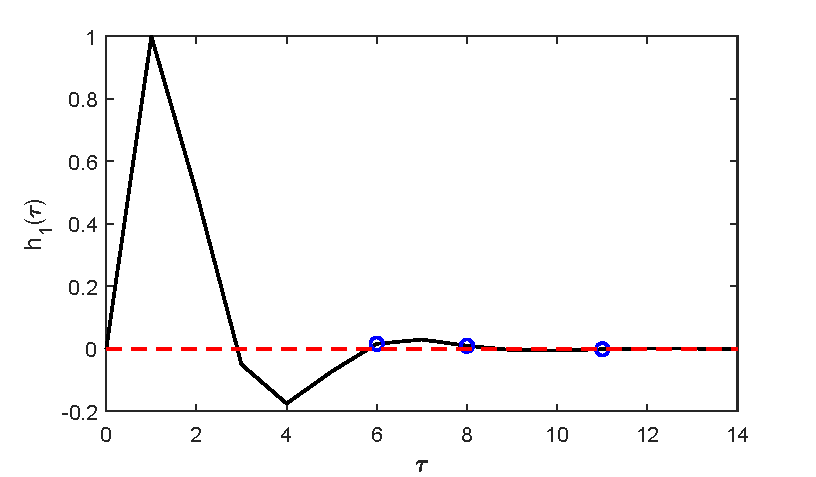
\includegraphics[width = 0.7\textwidth]{Chapter4_EM/LinearKernel_EM.pdf}
\caption{The true first order kernel $h_1$ (black line) in the simulation example, and the three applied truncation lengths (blue circles)}
\label{fig:LinearKernel_EM}
\end{figure}

For both tuning methods, hyperparameters are initialized according to,
%\begin{align*}
%&[\hat{\sigma}^2]^{(0)} = 1.5\sigma^2 \\
%&\hat{c}_m^{(0)} = 1 \; \; \forall \; m, \\
%&[\hat{\lambda}_m^j]^{(0)} = 0.8 \; \; \forall \; m,j.
%\end{align*}
$$ [\hat{\sigma}^2]^{(0)} = 1.5\sigma^2, \; \; \; \hat{c}_m^{(0)} = 1, \; \; \; [\hat{\lambda}_m^j]^{(0)} = 0.8 \; \; \forall \; m,j$$
All non-convex optimizations are performed using $\text{\tt{fmincon}}$ in MATLAB, with a step tolerance of $10^{-3}$. Convergence of the iterative EM method is defined by a change of less than $1\%$ in all hyperparameters. Computation times are measured from the beginning of hyperparameter tuning to convergence, using a PC with Intel Xeon 3.50 GHz processor. In order to observe mean behaviour, each Monte Carlo study considers 10 realizations of each system.

\subsection{Results}

As well as computation time measurements, a validation error metric is calculated for each estimated system by applying a Gaussian validation input of length 20,000 to the estimated and true systems. Labeling the true output as $y_{val}$ and estimated output as $y_{est}$, we construct a normalized RMS error metric defined by,
\begin{equation}
E_{NRMS} = \frac{\text{rms}(y_{val}-y_{est})}{\text{rms}(y_{val})}.
\end{equation}

\renewcommand{\arraystretch}{1.3}
\begin{table}[!h]
\centering
\caption{Mean computation times and validation errors for $n_m = 7$}
\label{Results_nm7}
\begin{tabular}{l||r|r||r|r}
\hline
                & \multicolumn{2}{c||}{\textbf{Mean Comp. Time (s)}} & \multicolumn{2}{c}{\textbf{Mean E\textsubscript{NRMS}}} \\ \cline{2-5} 
\textbf{M} & \hspace{10mm} MLM          & EM            & \hspace{1mm} MLM             & EM            \\ \hline \hline 
1          & 0.064              & 0.173             & 0.249                & 0.224              \\ \hline
2          & 0.132               & 0.389             & 0.189                & 0.187              \\ \hline
3           & 2.848              & 2.114             & 0.176                & 0.161              \\ \hline
4          & 40.10               & 23.13            & 0.133                & 0.135              \\ \hline
5         & 501.9               & 217.7            & 0.117                & 0.114              \\ \hline
\end{tabular}
\end{table}

\renewcommand{\arraystretch}{1.3}
\begin{table}[!h]
\centering
\caption{Mean computation times and validation errors for $n_m = 9$}
\label{Results_nm9}
\begin{tabular}{l||r|r||r|r}
\hline
                & \multicolumn{2}{c||}{\textbf{Mean Comp. Time (s)}} & \multicolumn{2}{c}{\textbf{Mean E\textsubscript{NRMS}}} \\ \cline{2-5} 
\textbf{M} & \hspace{10mm} MLM           & EM            & \hspace{1mm} MLM             & EM            \\ \hline \hline 
1          & 0.071               & 0.269             & 0.218                & 0.203              \\ \hline
2          & 0.229               & 0.778             & 0.148               & 0.148              \\ \hline
3           & 8.704               & 7.761             & 0.123                & 0.120              \\ \hline
4          & 282.6               & 155.3            & 0.089                & 0.101              \\ \hline
5         & 3962              & 1523            & 0.071                & 0.085              \\ \hline
\end{tabular}
\end{table}

\renewcommand{\arraystretch}{1.3}
\begin{table}[!h]
\centering
\caption{Mean computation times and validation errors for $n_m = 12$}
\label{Results_nm12}
\begin{tabular}{l||r|r||r|r}
\hline
                & \multicolumn{2}{c||}{\textbf{Mean Comp. Time (s)}} & \multicolumn{2}{c}{\textbf{Mean E\textsubscript{NRMS}}} \\ \cline{2-5} 
\textbf{M} & \hspace{10mm} MLM           & EM            & \hspace{1mm} MLM             & EM            \\ \hline \hline 
1          & 0.047               & 0.135             & 0.170                & 0.187              \\ \hline
2          & 0.476               & 1.387             & 0.116               & 0.120              \\ \hline
3           & 30.99               & 46.75             & 0.079                & 0.073              \\ \hline
4          & 2799               & 1211            & 0.059                & 0.060              \\ \hline
5         & 80000              & 15720            & 0.040                & 0.062              \\ \hline
\end{tabular}
\end{table}

The mean computation time results shown in Table \ref{Results_nm7} for $n_m = 7$, Table \ref{Results_nm9} for $n_m = 9$, and Table \ref{Results_nm12} for $n_m =12$, demonstrate that a dramatic improvement in computation time scaling is achieved using the proposed EM method for hyperparameter optimization. For the given experimental conditions, estimation time using EM is comparable to MLM tuning at 3rd order, and significantly faster for 4\textsuperscript{th} and higher order systems. The mean validation errors are also provided in the tables, confirming that there is no degradation in model quality. This is not surprising, since the hyperparameters were observed to converge to the same locations for both methods. Figure \ref{fig:EMhyperparams_converging} shows the EM convergence pathway for all hyperparameters in an example 2nd order ($M=2$) realization.

\begin{figure}[h]
\centering
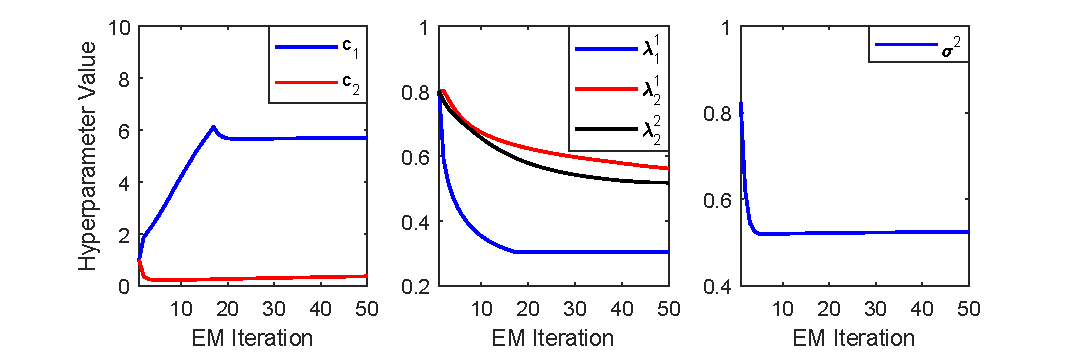
\includegraphics[width = \textwidth]{Chapter4_EM/HyperparamConvergence.pdf}
\caption{EM convergence pathway for all hyperparameters in a 2nd order example}
\label{fig:EMhyperparams_converging}
\end{figure}

To visualize the computation time trend, we label the $M$\textsuperscript{th} order mean computation times as $t_{EM}(M)$ and $t_{MLM}(M)$ for the EM and MLM methods respectively, and define the ratio function, 
\begin{equation}
R(M) = \frac{t_{EM}(M)}{t_{MLM}(M)}.
\end{equation}

$R(M)$ is plotted for all memory lengths in Figure \ref{fig:TimeRatio_EM}. Despite a significant difference in the number of parameters being estimated in each case, the relationship between $R(M)$ and $M$ remains similar, with a crossover point to EM superiority, in terms of computation time, at $M=3 \text{ or } 4$, depending on the memory length. Note that as $n_m$ increases, $R(3)$ increases while $R(M\geq4)$ decreases. The trend predicts increased relative benefit of EM over MLM tuning if $M$ and $n_m$ are increased further. 

\begin{figure}[h]
\centering
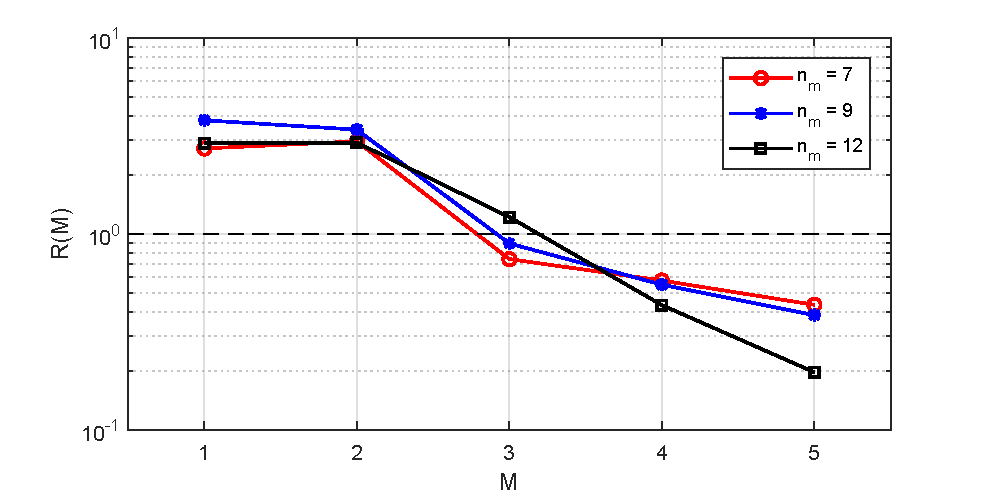
\includegraphics[width = 0.9\textwidth]{Chapter4_EM/Ratios_revised2.pdf}
\caption{Ratios of computation times for varying $M$ and $n_m$}
\label{fig:TimeRatio_EM}
\end{figure}

\section{Conclusion}

Bayesian regularization of Volterra kernel estimates necessitates the optimization of a large number of hyperparameters. When optimizing through a single global marginal likelihood maximization, the computational burden scales rapidly with the order of the Volterra series. In this chapter, the optimization problem was reformulated within an expectation-maximization framework. The new formulation splits the optimization into many small problems, some of which are analytic in nature. The remaining non-convex optimization problems have significantly reduced dimension and do not scale as rapidly with the order of the series. 

Evaluating the MLM and proposed EM-based tuning methods in a Monte-Carlo study revealed improved computation time scaling for the proposed method, with computation time for 4\textsuperscript{th} and 5\textsuperscript{th} order system estimates being significantly lower overall. In the studied example, validation errors obtained using each method's hyperparameters were very similar, and the EM hyperparameters were confirmed to be converging to a maximum of the marginal likelihood function. 